%!TEX root=paper/thesis.tex
\subsection{Reward definition}\label{sec:clf_reward}

\begin{figure}[ht]
\centering
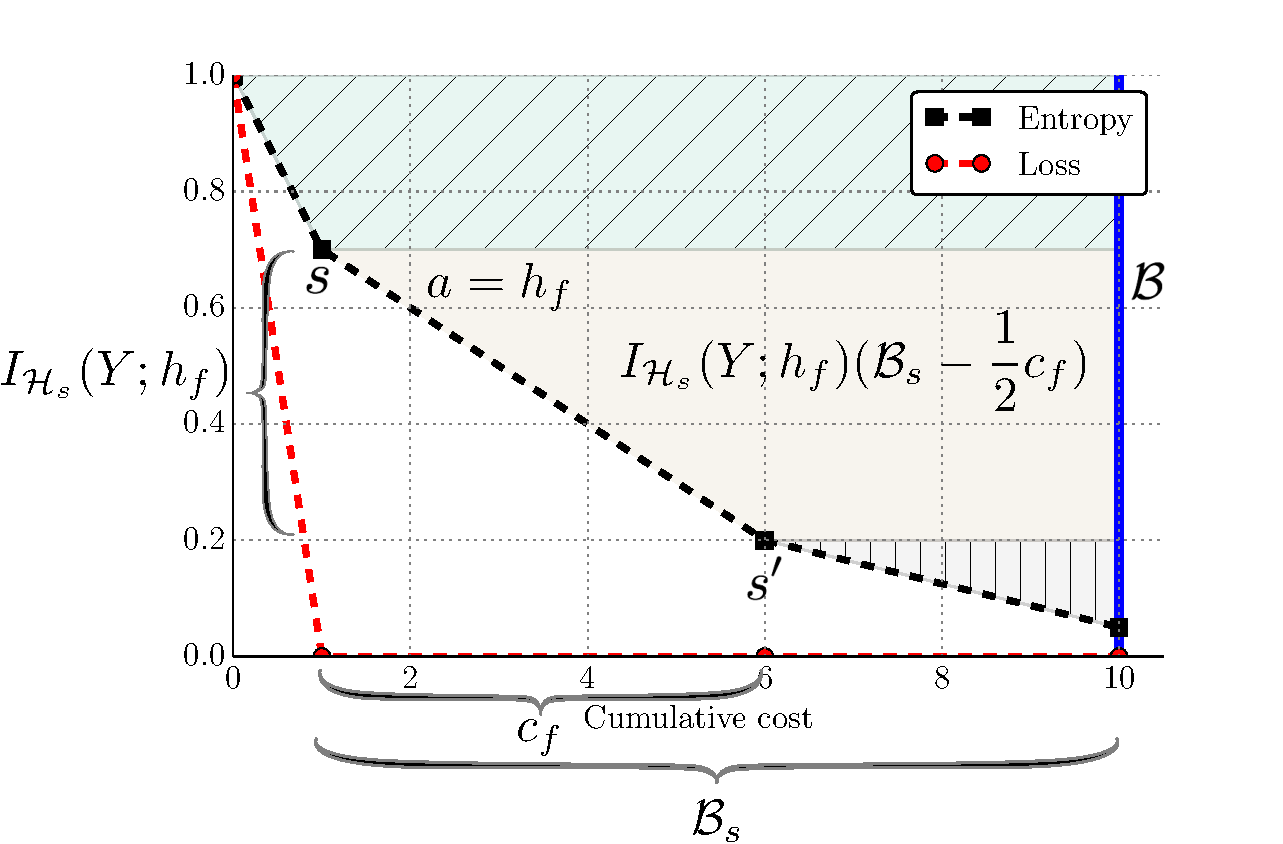
\includegraphics[width=.8\linewidth]{../../figures/rewards.pdf}
\caption{
Definition of the reward function.
To maximize the total area above the entropy vs. cost curve from $0$ to $\mathcal{B}$, we define the reward of an individual action as the area of the slice of the total area that it contributes.
From state $s$, action $a = h_f$ leads to state $s'$ with cost $c_f$.
The information gain is $I_{\mathcal{H}_s}(Y; h_f) = H(Y; \mathcal{H}_s) - H(Y; \mathcal{H}_s \cup {h_f})$.
\label{fig:clf_rewards}}
\end{figure}


The budget-sensitive loss $\mathcal{L}_\mathcal{B}$ enforces Anytime performance by valuing early gains more than later gains.
To formalize this, consider \hyperref[fig:clf_rewards]{Figure~\ref*{fig:clf_rewards}}, which shows the entropy and the 0-1 loss of $g$ at every point in a sequential feature selection episode for some instance $x$.
For the best Anytime performance, we want to capture the most area above the loss vs. cost curve, up to max budget $\mathcal{B}$ \parencite{Karayev-NIPS-2012}.

Recall from \eqref{eq:expected_reward} that the value of an episode $\xi$ is defined as the sum of obtained rewards.
If the reward of a single action is defined as the area above the curve that is captured as a direct result, then the value of the whole episode exactly corresponds to $\mathcal{L}_\mathcal{B}$.

However, there is a problem with using loss directly: only the first action to ``tip the scale'' toward the correct prediction gets a direct reward (in the figure, it is the first action).  A smoother reward function is desirable:
if the classifier $g$ can give a full distribution $P(Y = y \mid \mathcal{H}_{\pi(x)})$ and not just a prediction $\hat{y} \in \mathcal{Y}$, we can maximize the \emph{information gain} of the selected subset instead of directly minimizing the loss of $g(\pi(x))$:
\begin{eqnarray}
I(Y; \mathcal{H}_{\pi(x)}) &=& H(Y) - H(Y | \mathcal{H}_{\pi(x)}) = \\ \notag
&=& \sum_{y \in Y} P(y) \log P(y) -  \\ \notag
&&\sum_{y, \mathcal{H}_{\pi(x)}} P(y, \mathcal{H}_{\pi(x)}) \log P(y \mid \mathcal{H}_{\pi(x)})
\end{eqnarray}
To the extent that $g$ is unbiased, maximizing information gain corresponds to minimizing loss, and ensures that we not only make the right classification decision but also become maximally certain.
Therefore, as graphically presented in \hyperref[fig:clf_rewards]{Figure~\ref*{fig:clf_rewards}}, we define the reward of selecting feature $h_s$ with cost $c_f$ with the set $\mathcal{H}_s$ computed to be $I_{\mathcal{H}_s}(Y; h_f) (\mathcal{B}_s - \frac{1}{2}c_f)$.

\todo{In other words, the value of taking an action is the entire area above the curve as defined in \autoref{fig:clf_rewards}.}

Although we do not evaluate in this regime, note that this definition easily incorporates a \textbf{setup cost} in addition to \textbf{deadline cost} by only computing the area in between setup and deadline costs.
